\documentclass[]{article}

\usepackage[italian]{babel}
\usepackage[margin=20mm, footskip = 20pt]{geometry}
\usepackage{array}
\usepackage{tabularx}
\usepackage{graphicx}
\usepackage{subfiles}
\usepackage{hyperref}
\usepackage{nameref}
\usepackage{titlesec}
\usepackage{longtable}
\usepackage[table]{xcolor}
\usepackage{titling}
\usepackage{lastpage}
\usepackage{ifthen}
\usepackage{calc}
\usepackage{soulutf8}
\usepackage{contour}
\usepackage{float}
\usepackage{fancyhdr}
\usepackage{multirow}
\usepackage{pgfgantt}
\usepackage{lscape}

\newcommand{\hr}{\par\vspace{-.1\ht\strutbox}\noindent\hrulefill\par}

\graphicspath{ {./}
	{./commons/res}
}

%--------------------------------------------------
% Comandi per inserire contenuto del documento
%--------------------------------------------------
\makeatletter

\newcommand\appendToGraphicsPath[1]{%
	\g@addto@macro\Ginput@path{{#1}}%
}

\newcommand{\setTitle}[1]{%
	\newcommand{\@phTitle}{#1}%
}
\newcommand{\phTitle}{\@phTitle}

\newcommand{\setDate}[1]{%
	\newcommand{\@phDate}{#1}%
}
\newcommand{\phDate}{\@phDate}

\newcommand{\setUso}[1]{%
	\newcommand{\@uso}{#1}%
}
\newcommand{\uso}{\@uso}

\newcommand{\setVersione}[1]{%
	\newcommand{\@versione}{#1}%
}
\newcommand{\versione}{\@versione}

\newcommand{\disabilitaVersione}{%
	\renewcommand{\setVersione}[1]{}%
	\renewcommand{\versione}{DISABILITATA}
}

\newcommand{\setResponsabile}[1]{%
	\newcommand{\@responsabile}{#1}%
}
\newcommand{\responsabile}{\@responsabile}

\newcommand{\setRedattori}[1]{%
	\newcommand{\@redattori}{#1}%
}
\newcommand{\redattori}{\@redattori}

\newcommand{\setVerificatori}[1]{%
	\newcommand{\@verificatori}{#1}%
}
\newcommand{\verificatori}{\@verificatori}

\newcommand{\setModifiche}[1]{%
	\newcommand{\@modifiche}{#1}%
}
\newcommand{\modifiche}{\@modifiche}

\makeatother 

%--------------------------------------------------
% Comandi per i documenti esterni e il glossario
%--------------------------------------------------

\newcommand{\dext}[1]{\textsc{#1\textsubscript{\textit{D}}}}

\newcommand{\glock}[1]{\textsc{#1\textsubscript{\textit{G}}}}

%--------------------------------------------------
% Comandi per impostare sottotitoli di quarto e quinto livello
%--------------------------------------------------

\setcounter{secnumdepth}{4}
\setcounter{tocdepth}{4}

\titleformat{\paragraph}
{\normalfont\normalsize\bfseries}{\theparagraph}{1em}{}
\titlespacing*{\paragraph}{0pt}{2.25ex plus 1ex minus .2ex}{1.5ex plus .2ex}

\titleformat{\subparagraph}
{\normalfont\normalsize\bfseries}{\thesubparagraph}{1em}{}
\titlespacing*{\subparagraph}{0pt}{1.75ex plus 1ex minus .2ex}{.75ex plus .1ex}

\appendToGraphicsPath{../../commons/res/}

%------------------------------
%
% COMANDI DI CONFIGURAZIONE
%
%------------------------------

\setTitle{Norme di Progetto}

\setVersione{0.1.0}

\setDate{15-12-2020}

\setResponsabile{Paolo Scanferlato}

\setRedattori{
	Alessandro Chimetto\\&
	Valton Tahiraj\\&
}

\setVerificatori{Alessandro Chimetto}

\setUso{Interno}

\setModifiche{
	0.2.0 & Alessandro Chimetto		& Amministratore& 20-12-2020 & Aggiunto processo: Gestione della Configurazione\\
	0.1.0 & Alessandro Chimetto		& Verificatore	& 15-12-2020 & Verificata Introduzione\\
	0.1.0 & Valton Tahiraj 			& Redattore 	& 14-12-2020 & Aggiunto Introduzione \\
	0.0.0 & Alessandro Chimetto		& Verificatore	& 14-12-2020 & Verifica prima stesura\\
	0.0.0 & Valton Tahiraj 			& Redattore 	& 14-12-2020 & Prima stesura
}

\begin{document}
	% Direttive per la creazione del titolo tramite comando maketitle
\title{\huge \textsc{\phTitle{}} \\
	\vspace{11pt} \large \textsc{\phDate{}}}

\author{} % Non toccare
\date{} % Non toccare

%--------------------
% Frontespizio
%--------------------

% Logo del gruppo
\begin{figure}[t!]
	\centering
	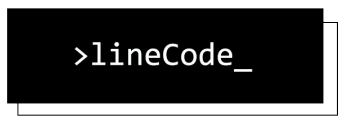
\includegraphics[width=20em]{lclong}
\end{figure}

% Titolo / Nome
\maketitle
\thispagestyle{empty}

% Dati specifici sul doc in forma tabulare
\begin{table}[ht]
	\begin{center}
		\label{tab:Dati sul documento}
		\begin{tabular}{r|l}
			\multicolumn{2}{c}{ \textsc{Dati sul documento} } \\
			\hline
			\textbf{Versione} & \versione{} \\
			\textbf{Uso} & \uso{}  \\
			\textbf{Redattori} & \redattori{} \\
			\textbf{Verificatori} & \verificatori{} \\
			\textbf{Responsabile} & \responsabile{} \\
			\textbf{Destinatari} & lineCode \\
								& prof.\ Vardanega Tullio \\		
								& prof.\ Cardin Riccardo \\
			\ifthenelse{\equal{\uso}{Esterno}}{
								& Sanmarco Informatica
			}{} \\
		\end{tabular}
	\end{center}
\end{table}

\newpage

\renewcommand{\arraystretch}{2} % allarga le righe con dello spazio sotto e sopra
\begin{longtable}[H]{>{\centering\bfseries}m{2cm} >{\centering}m{3.5cm} >{\centering}m{2.5cm} >{\centering}m{3cm} >{\centering\arraybackslash}m{5cm}}
	\rowcolor{lightgray}
	{\textbf{Versione}} & {\textbf{Nominativo}} & {\textbf{Ruolo}} & {\textbf{Data}} & {\textbf{Descrizione}}  \\
	\endfirsthead%
	\rowcolor{lightgray}
	{\textbf{Versione}} & {\textbf{Nominativo}}  & {\textbf{Ruolo}} & {\textbf{Data}} & {\textbf{Descrizione}}  \\
	\endhead%
	\modifiche{}%
\end{longtable}
	\newpage
	%--------------------------------
	%
	% IL CONTENUTO INIZIA DA QUI
	%
	%--------------------------------
	\section{Introduzione}
		\subsection{Scopo del documento}
		Il documento ha lo scopo di definire le guidelines del way of working adottato dal team lineCode. Le attività presenti in questo documento sono redatte da processi contenuti nello standard ISO/IEC 12207:1995. Risulta quindi necessario che tutti i membri del gruppo prendano visione di questo documento ai fini di coesione e uniformità all'interno del progetto.

		\subsection{Scopo del Prodotto}
		Il \glock{capitolato} C5 ha come obbiettivo la realizzazione di un applicativo \glock{Real-Time} in grado di guidare delle unità dotate di mobilità autonoma in ambienti specifici, partendo dal presupposto che queste si muovano in ambienti in cui sono presenti altre unità (autonome o meno).

		\subsection{Glossario e documenti esterni}
		In supporto alla documentazione viene fornito un glossario per chiarire, con una definizione, eventuali termini specifici contenuti in questo documento.
		Saranno adottati quindi questi due simboli a pedice:
		\begin{itemize}
			\item \textit{D} se indicano un documento specifico;
			\item \textit{G} se incluse nel \dext{glossario}.
		\end{itemize}

		\subsection{Riferimenti}
			\subsubsection{Riferimenti Normativi}
			\begin{itemize}
				\item \textbf{{\glock{capitolato} C5 - PORTACS}}: \url{https://www.math.unipd.it/~tullio/IS-1/2020/Progetto/C5.pdf};
			\end{itemize}
			\subsubsection{Rifermenti informativi}
			\begin{itemize}
				\item \textbf{ISO/IEC 12207:1995}: \url{https://www.math.unipd.it/~tullio/IS-1/2009/Approfondimenti/ISO_12207-1995.pdf}
				\item \textbf{Semantic Versioning 2.0.0}: \url{https://semver.org/spec/v2.0.0.html}.
				\item \textbf{\dext{Studio di Fattibilità}};
				\item \textbf{\dext{Piano di Qualifica}};
				\item \textbf{\dext{Piano di Progetto}}.
			\end{itemize}

	\newpage

	\section{Processi di Supporto}
		\subsection{Gestione della Configurazione}
			\subsubsection{Obiettivi}
			Si vuole creare un ambiente di lavoro che sia comune a tutti i partecipanti al progetto e che permetta di applicare procedure amministrative e tecniche per tutta la durata del ciclo di vita del software. Più nello specifico si vuole consentire al programmatore di apportare modifiche al software e alla documentazione in modo asincrono rispetto agli altri membri del gruppo di lavoro. Per avere memoria storica delle modifiche effettuate, si vuole che queste vengano tracciate dall'ambiente di lavoro. In particolare, è d'interesse conoscere per ogni modifica:
			\begin{itemize}
				\item quale modifica è stata apportata;
				\item perché la modifica è stata apportata;
				\item quando è avvenuta la modifica;
				\item chi ha effettuato la modifica;
				\item in che parte del documento la modifica agisce.
			\end{itemize}
			Si vuole, inoltre, fare in modo che la modifica venga apportata solo se prima verificata da un verificatore di cui dovrà essere tracciata l'attività di verifica dall'ambiente di lavoro. Si vuole, infine, fare in modo che il responsabile possa monitorare l'andamento del progetto tramite sistemi di reportistica.

			\subsubsection{Documentazione come Software}
			Per favorire la tracciabilità delle modifiche alla documentazione, quest'ultima sarà costruita in linguaggio \glock{\LaTeX}\ e dunque le norme applicate a questo processo concernenti il software saranno applicate in egual modo alla documentazione tranne dove specificato diversamente in modo esplicito.

			\subsubsection{Strumenti di supporto}
			Gli strumenti utilizzati per garantire il \glock{workflow} sono:
			\begin{itemize}
				\item \textbf{\glock{git}}: come \glock{DVCS};
				\item \textbf{\glock{GitHub}}: per \glock{repository} remota, \glock{pull-request}, \glock{code-review} e \glock{CI} tramite \glock{GitHub Action};
				\item \textbf{\glock{GitKraken}}: come client git locale utilizzato da tutti i membri del gruppo;
				\item \textbf{\glock{Discord}}: come sistema di messaggistica e videoconferenza fra i membri del gruppo;
				\item \textbf{\glock{Zapier}}: per implementare automazioni fra \glock{GitHub} e \glock{Discord}.
			\end{itemize}

			\subsubsection{\glock{Workflow}}
			L'amministratore configura e mantiene un Distributed Version Control System (o \glock{DVCS}) che metta a disposizione una \glock{repository} remota in cui sarà presente il software. Sulla repository verrà effettuato un ciclo tale per cui ad ogni iterazione corrisponda l'integrazione di una nuova modifica. Ogni iterazione si compone dei seguenti passi:
			\begin{enumerate}
			\item il programmatore apporta la modifica in un \glock{branch} separato dal ramo principale, in modo asincrono rispetto ai colleghi; ogni \glock{commit} traccia le modifiche in modo conforme agli obiettivi;
			\item completata la modifica, il programmatore crea una \glock{pull-request} per richiedere l'integrazione della sua modifica;
			\item un'automazione (impostata inizialmente dall'amministratore) invia un messaggio nel sistema di messaggistica utilizzato dal gruppo di lavoro per avvisare i verificatori dell'avvenuta \glock{pull-request};
			\item il verificatore prende in carico la \glock{pull-request} rispondendo al messaggio inviato dall'automazione ed eseguendo l'attività di verifica della modifica proposta; il programmatore non può aggiungere \glock{commit} al proprio \glock{branch} una volta che il verificatore comunica l'inizio della sua attività rispondendo al messaggio automatico (a meno di un accordo fra di essi);
			\item nel caso in cui la modifica proposta non venga accettata, il verificatore utilizzerà il sistema di \glock{code-review} messo a disposizione dal \glock{VCS} per informare il programmatore sui cambiamenti da effettuare al fine di rendere la modifica adatta all'integrazione; il programmatore risponderà apportando i cambiamenti richiesti in un nuovo \glock{commit} sullo stesso \glock{branch};
			\item qualora la modifica proposta sia ritenuta accettabile dal verificatore, questo effettuerà la procedura di \glock{merge} nel ramo principale ed eliminerà il ramo creato dal programmatore (entrambe le operazioni vengono tracciate dal \glock{VCS});
			\item un'automazione, parte del sistema di Continuous Integration (o \glock{CI}), specifica per il prodotto contenuto nella repository, verrà eseguita automaticamente sul ramo principale per verificare che l'integrazione tramite \glock{merge} sia andata a buon fine con controlli automatici e report.
			\end{enumerate}

			\subsubsection{Codice di Versionamento}
			Si utilizza il seguente codice:
			\[
				\text{v}[\alpha].[\beta].[\gamma]
			\]
			\begin{itemize}
				\item \([\alpha]\): parte da 0 e non si resetta mai;
				\item \([\beta]\): parte da 0 e si resetta solo ad incrementi di \([\alpha]\);
				\item \([\gamma]\): parte da 0 e si resetta solo ad incrementi di \([\alpha]\) o \([\beta]\).
			\end{itemize}
			Il codice assume significato diverso in caso si tratti di documentazione o software:
			\begin{itemize}
				\item documentazione:
				\begin{itemize}
					\item \([\alpha]\): numero identificativo del rilascio del documento; viene incrementato solo dal responsabile a seguito di una approvazione quando il documento è pronto per essere rilasciato;
					\item \([\beta]\): avanzamento rispetto alle sezioni; viene incrementato dal programmatore quando aggiunge una nuova sezione al documento;
					\item \([\gamma]\): avanzamento rispetto a piccole migliorie; viene incrementato dal programmatore quando svolge piccole correzioni ortografiche o di sintassi in \LaTeX.
				\end{itemize}

				\item software:
				\begin{itemize}
					\item \([\alpha]\): numero identificativo della \glock{major release}; viene incrementato solo dopo aver implementato tutti i requisiti obbligatori;
					\item \([\beta]\): numero identificativo della \glock{minor release}; viene incrementato solo dopo l'implementazione di uno o più requisiti;
					\item \([\gamma]\): numero identificativo della \glock{patch}; viene incrementato in seguito a piccole modifiche (es. risoluzione di piccoli errori).
					\end{itemize}
			\end{itemize}

			\subsubsection{\glock{Repository} e relativa struttura}
			Ogni repository, sulla propria \glock{root}, contiene:
			\begin{itemize}
				\item \verb!.gitignore!: vi sono specificati tutti i file (o tipi di file) che non devono essere tracciati dal sistema di versionamento (es. file eseguibili);
				\item \verb!.github!: contiene file di configurazione specifici per \glock{GitHub} come le configurazioni per \glock{GitHub Action}.
			\end{itemize}
			Specifiche repository possiedono una struttura specifica:
				\paragraph{docs}
				Contiene la documentazione del progetto e si compone delle seguenti cartelle:
				\begin{itemize}
					\item \verb!commons/!: contiene configurazioni e risorse comuni a tutti i documenti;
					\item \verb!esterni/!: contiene tutta la documentazione esterna;
					\item \verb!interni/!: contiene tutta la documentazione interna.
				\end{itemize}

\end{document}
